\newpage
\section{Auswertung}

\subsection{Bestimmung des magnetischen Momentes unter Ausnutzung der Gravitation}
Die in dieser Methode eingestellten Ströme und gemessenen Abstände $r$ sind in Tabelle \eqref{tab:tabellegravmethode} zu finden. Die zu 
den Strömen gehörigen Flussdichten $B$ können mithilfe von Formel \eqref{eq:flussdichte} berechnet werden.

\begin{table}[htbp]
\centering
\caption{Gravitationsmethode: Ermittelte Größen}
\label{tab:tabellegravmethode}
\begin{tabular}{S[table-format=1.1] S[table-format=2.2] S[table-format=1.1]}
\toprule
 {$I/\, \symup{A}$} & {$B/10^{-3}\, \symup{T}$} & {$r/10^{-2}\, \symup{m}$} \\
\midrule
2.0 &  2.72 & 2.7 \\
2.3 &  3.13 & 3.5 \\
2.5 &  3.40 & 4.7 \\
2.6 &  3.54 & 4.5 \\
2.8 &  3.81 & 5.9 \\
3.0 &  4.08 & 4.2 \\
3.2 &  4.35 & 7.6 \\
3.5 &  4.76 & 7.3 \\
3.7 &  5.03 & 8.8 \\
4.0 &  5.44 & 9.3 \\

\bottomrule
\end{tabular}
\end{table}

Es wird nun $r$ gegen $B$ aufgetragen wie in Abbildung \eqref{fig:bildgravmethode} zu sehen ist.
\begin{figure}[h!]
\centering
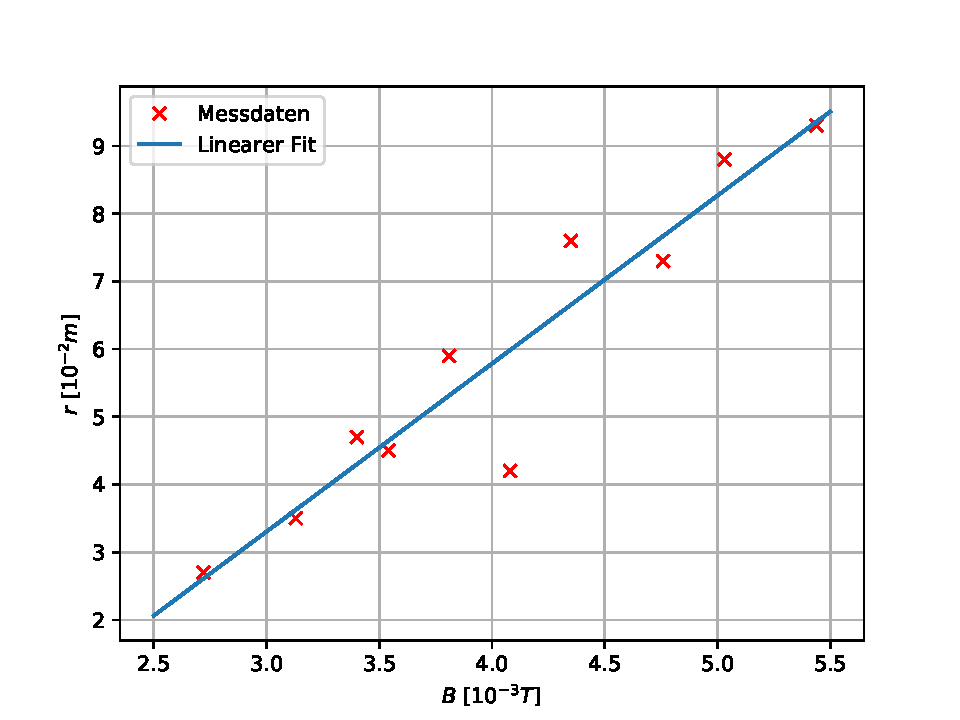
\includegraphics[scale=.9]{GravMethode.pdf}
\caption{Lineare Regression zur Bestimmung des magnetischen Moments über die Gravitation.}
\label{fig:bildgravmethode}
\end{figure}
Die Steigung der Ausgleichsgeraden der Form $y = a\cdot x + b$ wird vom Python-Modul Matplotlib berechnet und beträgt 
\begin{equation*}
a = \frac {r}{B}= (24{,}816 \pm 3{,}018)\, \symup{\frac{m}{T}}
\end{equation*}
und der y-Achsenabschnitt liegt bei
\begin{equation*}
b = (-0{,}041 \pm 0{,}012)\, \symup{m}.
\end{equation*}
Mit dem Gewicht der kleinen Masse $m$ von $m = 0{,}0014\, \symup{kg}$ und der Erdbeschleunigung g, welche hier 
$g = 9{,}81\, \symup{\frac{m}{s^2}}$ ist, lässt sich so ein magnetisches Moment $\mu_{\text{Dipol}}$ über Gleichung \eqref{eq:udipol} 
berechnen.
Da es sich bei $a$ um eine fehlerbehaftete Größe handelt, wird der Fehler $\Delta{\mu_{\text{Dipol}}}$ des magnetischen Momentes mithilfe der Gauß'schen 
Fehlerfortpflanzung berechnet.
\begin{equation*}
\begin{aligned}
\Delta{\mu_{\text{Dipol}}} &= \sqrt{\biggl(\frac{\partial \mu_{\text{Dipol}}}{\partial a}\biggr)^2 \cdot (\Delta a)^2} \\
\implies \Delta{\mu_{\text{Dipol}}} &= \sqrt{(m \cdot g)^2 \cdot (\Delta a)^2} \\
\end{aligned}
\end{equation*}

\begin{equation}
\iff \Delta{\mu_{\text{Dipol}}} = m \cdot g \cdot \Delta a
\label{eq:gravfehler}
\end{equation}
Werden nun alle Werte in Gleichung \eqref{eq:udipol} sowie in \eqref{eq:gravfehler} eingesetzt, ergibt sich ein magnetisches
Moment von
\begin{equation*}
\mu_{\text{Dipol}} = (0{,}34 \pm 0{,}04)\, \symup{A \cdot m^2}.
\end{equation*}



%-----------------------------------------------------

\subsection{Bestimmung des magnetischen Momentes über die Schwingungsdauer}
In diese Messmethode wird das magnetische Moment $\mu_{\text{Dipol}}$ über Gleichung \eqref{eq:Schwingungsdauer} ermittelt. 
Das hierfür benötigte Trägheitsmoment $J_{\text{K}}$ der im Versuch verwendeten Billiardkugel mit den Geometriedaten 
\begin{equation*}
\begin{aligned}
r_{\text{K}} &= 2{,}5\, \symup{cm}, \\
m_{\text{K}} &= 150\,\symup{g}
\end{aligned}
\end{equation*}
wird mit 
\begin{equation*}
J_{\text{K}} = \frac{2\cdot m_{\text{K}} \cdot r^2_{\text{K}}}{5}
\end{equation*}
bestimmt. Das Trägheitsmoment beträgt damit 
\begin{equation*}
J_{\text{K}} = 3,75 \cdot 10^{-5} \, \symup{kg m^2}.
\end{equation*}

\newpage

In Tabelle \eqref{tab:tabelleschwingung} sind die eingestellten Ströme sowie die gemessenen Periodendauern zu finden.
\begin{table}[htbp]
\centering
\caption{Schwingungsmethode: Ermittelte Größen}
\label{tab:tabelleschwingung}
\begin{tabular}{S[table-format=1.1] S[table-format=1.2] S[table-format=3.2] S[table-format=1.3] S[table-format=1.3]}
\toprule
 {$I/\symup{A}$} & {$B/10^{-3}\symup{T}$} & {$\frac{1}{B}/\frac{1}{T}$} & {$T/s$} & {$T^2/s^2$} \\
\midrule
2.0 &  2.72 & 367.65 & 1.172 & 1.374 \\
2.3 &  3.13 & 319.49 & 1.106 & 1.223 \\
2.5 &  3.40 & 294.12 & 1.053 & 1.109 \\
2.6 &  3.54 & 282.49 & 1.038 & 1.077 \\
2.8 &  3.81 & 262.47 & 0.991 & 0.982 \\
3.0 &  4.08 & 245.09 & 0.963 & 0.927 \\
3.2 &  4.35 & 229.89 & 0.931 & 0.867 \\
3.5 &  4.76 & 208.77 & 0.897 & 0.805 \\
3.7 &  5.03 & 198.81 & 0.860 & 0.739 \\
4.0 &  5.44 & 183.82 & 0.768 & 0.589 \\

\bottomrule
\end{tabular}
\end{table}
Nun wird $T^2$ gegen $\frac{1}{B}$ aufgetragen wie in Abbildung \eqref{fig:bildschwingung} zu sehen ist.

\begin{figure}[h!]
\centering
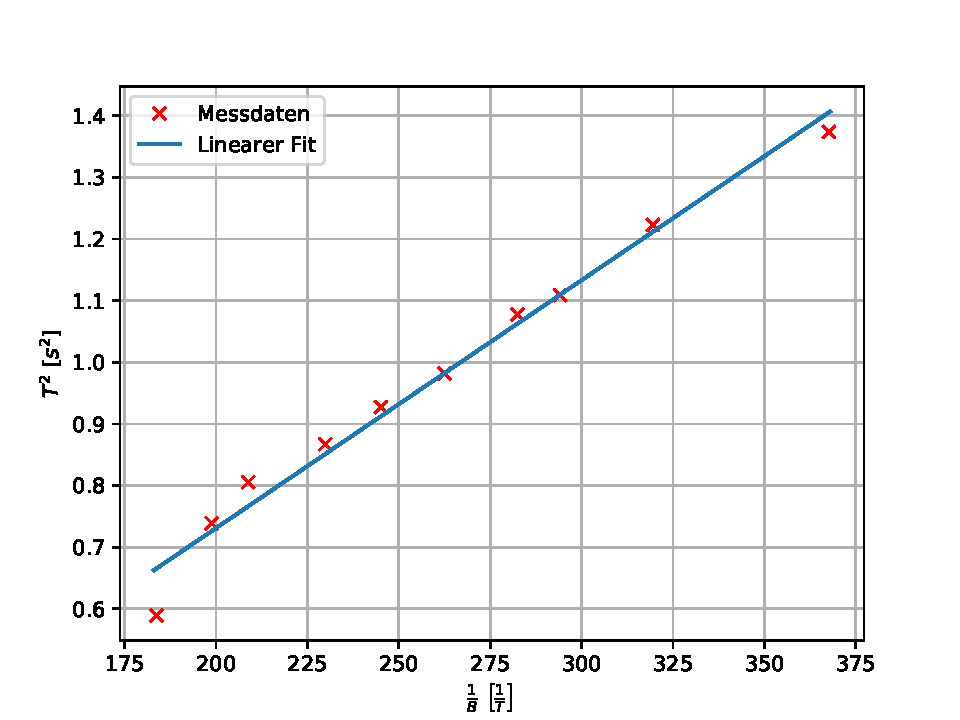
\includegraphics[scale=.9]{SchwingungsMethode.pdf}
\caption{Lineare Regression zur Bestimmung des magnetischen Moments über die Schwingungsdauer.}
\label{fig:bildschwingung}
\end{figure}

Die von Matplotlib berechnete Steigung der Ausgleichgeraden der Form $y = a \cdot x + b$ beträgt 
\begin{equation*}
a = T^2\cdot B = (0{,}00402 \pm 0{,}00019)\, \symup{s^2\cdot T}, 
\end{equation*}
der Y-Achsenabschnitt ist 
\begin{equation*}
b = (-0{,}07 \pm 0{,}05)\, \symup{s^2}. 
\end{equation*}

Der Fehler $\Delta \mu_{\text{Dipol}}$ des magnetisches Moments wird über die Gauß'sche Fehlerfortpflanzung ermittelt:
\begin{equation*}
\begin{aligned}
\Delta{\mu_{\text{Dipol}}} &= \sqrt{\biggl(\frac{\partial \mu_{\text{Dipol}}}{\partial a}\biggr)^2 \cdot (\Delta a)^2} \\
\implies \Delta{\mu_{\text{Dipol}}} &= \sqrt{\biggl(- \frac{4\pi^2 \cdot J_{\text{K}}}{a^2}\biggr)^2 \cdot (\Delta a)^2} \\
\end{aligned}
\end{equation*}
\begin{equation}
\iff \Delta{\mu_{\text{Dipol}}} = \frac{4\pi^2 \cdot J_{\text{K}}}{a^2} \cdot \Delta a
\label{eq:schwingungsfehler}
\end{equation}

Nach Einsetzen der Werte für $J_{\text{K}}$, $a$ und $\Delta a$ in Gleichung \eqref{eq:Schwingungsdauer} und \eqref{eq:schwingungsfehler}
folgt für das magnetische Moment:
\begin{equation*}
\mu_{\text{Dipol}} = (0{,}368 \pm 0{,}017)\, \symup{A \cdot m^2}.
\end{equation*}



%-----------------------------------------------------
\newpage
\subsection{Bestimmung des magnetischen Moments über die Präzession}
Mit Gleichung \eqref{eq:Praezession} kann $\mu_{\text{Dipol}}$ über die Präzessionsmethode berechnet werden. Der Drehimpuls $L_{\text{K}}$ ist
\begin{equation}
L_{\text{K}} = J_{\text{K}} \cdot 2\pi \nu.
\label{eq:drehimpuls}
\end{equation}
Das Trägheitsmoment mit $J_{\text{K}} = 3{,}75 \cdot 10^{-5} \, \symup{kgm^2}$ und die Frequenz, welche $\nu = 5{,}8\, \symup{Hz}$ 
beträgt, können in \eqref{eq:drehimpuls} eingesetzt werden. Der Drehimpuls ist damit
\begin{equation*}
L_{\text{K}} = 1{,}367\cdot 10^{-3}\, \symup{\frac{kg\cdot m^2}{s}}.
\end{equation*}

Aus Tabelle \eqref{tab:tabellepraezi} können die Ströme $I$, die daraus resultierenden magnetischen Flussdichten $B$ und die 
Periodendauern $T$ entnommen werden. Weiterhin enthält sie die gemittelten Periodendauern $\bar{T}$ sowie die 
Kehrwerte $\frac{1}{\bar{T}}$. Der Mittelwert wird hierbei mit
\begin{equation*}
\bar{T} = \frac{1}{N} \sum_{\mathclap{i=1}}^N T_{\text{i}}
\end{equation*}
und der zugehörige Fehler mit
\begin{equation*}
\Delta\bar{T} = \frac{1}{\sqrt{N}} \sqrt{\frac{1}{N-1}\sum_{\mathclap{i=1}}^N (T_{\text{i}}-\bar{T})^2}
\end{equation*}
berechnet.
Der Fehler der gemittelten, reziproken Periodendauern $\frac{1}{\bar{T}}$ wird weiterhin mithilfe der Gauß'schen Fehlerfortpflanzung kalkuliert:

\begin{equation*}
\begin{aligned}
\Delta{\frac{1}{\bar{T}}} &= \sqrt{\biggl(\frac{\partial \frac{1}{\bar{T}}}{\partial \bar{T}}\biggr)^2 \cdot (\Delta \bar{T})^2} \\
\implies \Delta{\frac{1}{\bar{T}}} &= \sqrt{\biggl( - \frac{1}{\bar{T}^2}\biggr)^2 \cdot (\Delta \bar{T})^2} \\
\iff \Delta{\frac{1}{\bar{T}}} &= \frac{\Delta \bar{T}}{\bar{T}^2}. \\
\end{aligned}
\end{equation*}


\begin{table}[htbp]
\centering
\caption{Präzessionsmethode: Ermittelte Größen}
\label{tab:tabellepraezi}
\begin{tabular}{S[table-format=1.1] S[table-format=1.2] S S S[table-format=2.2] S[table-format=2.3, table-figures-uncertainty=1] S[table-format=2.4, table-figures-uncertainty=1]}
\toprule
 {$I/\symup{A}$} & {$B/10^{-3}\symup{T}$} & {$T_1/\symup{s}$} & {$T_2/\symup{s}$} & {$T_3/\symup{s}$} & {$\bar{T}/\symup{s}$} & {$\frac{1}{\bar{T}}/\symup{10^2 s}$}\\
\midrule
0.5 &  0.68 & 25.28 & 25.06 & 20.88 & 23.70 \pm 0.4 & 4.2194 \pm 0.0007\\
1.0 &  1.36 & 12.88 & 15.15 & 15.75 & 14.60 \pm 0.2 & 6.8493 \pm 0.0009\\
1.5 &  2.04 & 10.06 &  8.13 &  8.60 &  8.93 \pm 0.15 & 11.1982 \pm 0.0018\\ 
2.0 &  2.72 &  8.31 &  8.04 &  7.50 &  7.95 \pm 0.06 & 12.5786 \pm 0.0009\\
2.5 &  3.40 &  6.69 &  5.91 &  5.90 &  6.16 \pm 0.07 & 16.2338 \pm 0.0018\\
2.7 &  3.67 &  6.59 &  6.69 &  7.29 &  6.86 \pm 0.05 & 14.5573 \pm 0.0011\\
3.0 &  4.08 &  4.62 &  5.78 &  6.06 &  5.486 \pm 0.114 & 18.228 \pm 0.003\\
3.5 &  4.76 &  4.66 &  5.09 &  4.59 &  4.78 \pm 0.04 & 20.9205 \pm 0.0018\\
3.7 &  5.03 &  4.69 &  4.37 &  5.09 &  4.72 \pm 0.05 & 21.186 \pm 0.002\\
4.0 &  5.44 &  5.00 &  4.81 &  4.50 &  4.77 \pm 0.04 & 20.9644 \pm 0.0018\\

\bottomrule
\end{tabular}
\end{table}
\begin{figure}[h]
\centering
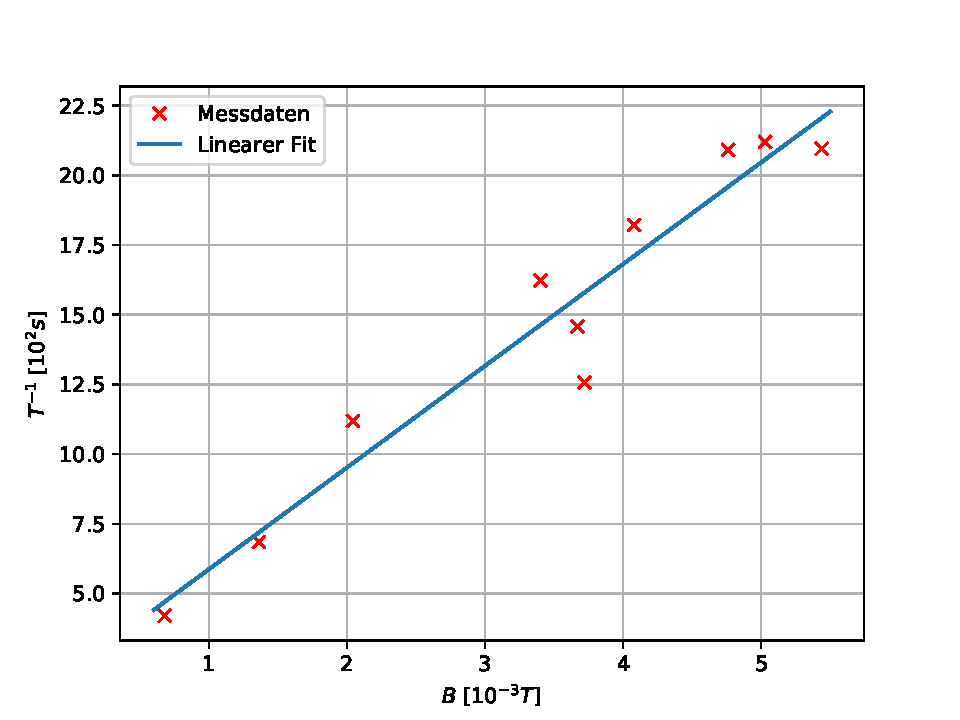
\includegraphics[scale=.9]{PraezessionsMethode.pdf}
\caption{Lineare Regression zur Bestimmung des magnetischen Moments über die Präzession}
\label{fig:bildpraezi}
\end{figure}
In Abbildung \eqref{fig:bildpraezi} werden die gemittelten, reziproken Periodendauern $\frac{1}{\bar{T}} = T_{\text{p}}$ gegen die magnetischen 
Flussdichten aufgetragen. 
Aus der linearen Regression der Form $y=a\cdot x +b$ ergibt sich die Steigung $a$ und der y-Achsenabschnitt $b$, welche wiederum von Matplotbib ausgegeben werden:
\begin{equation*} 
\begin{aligned}
a = \frac{1}{T_{\text{p}} \cdot B} &= (36{,}5 \pm 3{,}4)\, \symup{\frac{1}{s\cdot T}}, \\
b &= (2{,}2 \pm 1{,}3)\cdot 10^2 \, \symup{s}. 
\end{aligned} 
\end{equation*}

Für den Fehler $\Delta \mu_{\text{Dipol}}$ des magnetischen Moments wird die Gauß'sche Fehlerfortpflanzung genutzt:
\begin{equation*}
\begin{aligned}
\Delta{\mu_{\text{Dipol}}} &= \sqrt{\biggl(\frac{\partial \mu_{\text{Dipol}}}{\partial a}\biggr)^2 \cdot (\Delta a)^2} \\
\implies \Delta{\mu_{\text{Dipol}}} &= \sqrt{\biggl( 2\pi \cdot L_{\text{K}}\biggr)^2 \cdot (\Delta a)^2} \\
\end{aligned}
\end{equation*}
\begin{equation}
\iff \Delta{\mu_{\text{Dipol}}} = 2\pi \cdot L_{\text{K}} \cdot \Delta a
\label{eq:praezessionsfehler}
\end{equation}

Nach Einsetzen von $L_{\text{K}}$, $a$ und $\Delta a$ in Gleichung \eqref{eq:Praezession}, sowie \eqref{eq:praezessionsfehler} ergibt sich ein magnetisches Moment von
\begin{equation*}
\mu_{\text{Dipol}} = (0{,}31 \pm 0{,}03)\, \symup{A \cdot m^2}.
\end{equation*}
